\hypertarget{towards-manipulable-models}{%
\chapter{Towards Manipulable Models}\label{towards-manipulable-models}}

\usetikzlibrary{positioning,arrows,calc}
\tikzset{
    graph/.style={>=stealth,shorten >=1pt,shorten <=1pt,auto,node distance=1.5cm, semithick},
    world/.style={circle,draw,minimum size=0.5cm,fill=gray!15}, point/.style={circle,draw,inner sep=0.5mm,fill=black},
    model/.style={circle,draw,minimum size=0.5cm,fill=gray!20}, point/.style={circle,draw,inner sep=0.5mm,fill=black},
    reflexive above/.style={->,loop,looseness=7,in=120,out=60},
    reflexive below/.style={->,loop,looseness=7,in=240,out=300},
    reflexive left/.style={->,loop,looseness=7,in=150,out=210},
    reflexive right/.style={->,loop,looseness=7,in=30,out=330}
}

Before diving into Zollman's models, I want to clarify precisely what I
mean by model and define other relevant terms. I discuss models because
my specific understanding of models is a key motivation for my
experimental work. This section touches on the vibrant debate about the
role of models in science and I, for the most part, try to stick to
fairly widespread theories and understandings. However, in certain
areas, I extend and combine these understandings to create a more
complete account of the issues salient for Zollman's computational
modeling. To this end, I will build a case for viewing computational
models as mechanisms that can be studied through experimentation in the
same way biological mechanisms are studied.

Through this lens, a computational model can be viewed in the same
manner that a lab rat might be viewed as a model of a person for
conducting biomedical research. Manipulating the computational model's
mechanism can generate an explanation for the model's phenomena much
like an experiment performed on a rat generates an explanation for some
phenomena observed on the rat. If these explanations hold up on the rat,
so long as there is good reason to believe the model mechanism behaves
like the mechanism being modeled, we should have good reason to believe
the explanation holds up on the target of study.

Because simulations are generally fairly easy to manipulate relative to
many targets of scientific inquiry, such as humans or the climate,
simulations are particularly suited to exploratory research. In the
exploratory mode of research, there might not be hard and fast
hypotheses as research might focus more on determining which hypotheses
might be worth testing in the first place. If hypothesis-based research
is about verifying that the hypothesis is true or not, exploratory
research is about finding promising ideas. This exploratory phase
benefits from a high degree of trial and error, which simulations
uniquely enable by lowering the barrier to trying many different
manipulations of a model to quickly get a feel for what works and what
doesn't.

This mode is particularly important for productive scientific inquiry
where definitive hypothesis testing is expensive, difficult, or even
impossible. For example, by the clinical trial phase of drug
development, a drug candidate must be promising and worthy of expensive
clinical trials to determine if their observed effect is indeed real and
that unintended side-effects are not present. To gain enough confidence
in the candidate drug to advance it to this stage, researchers perform
quite a bit of exploratory testing on animal models, such as rats or
mice, to determine which specific compounds seem worthy of the
investment of hypothesis testing.

I argue that simulations can be particularly useful within the
exploratory. Simulations, when done well, provide a unique way to
manipulate what would otherwise be difficult to manipulate and allow for
more trial and error in the exploratory phase of research. This
additional trial and error, in turn, should result in better hypotheses
and better science because the simulation allows for many more
experiments to be carried out. While these simulations are certainly not
perfect representations of their target, this isn't strictly necessary
for them to be valuable at the exploratory stage. Mice aren't exactly
like humans but are still hugely valuable experimental models for
exploring new biomedical interventions on humans.

To reach this conclusion, I'll first describe traditional approaches to
understanding models in science as well as extensions of those theories
to simulations and computational models. I'll then give a brief account
of how mechanisms lead to explanations under the manipulability account
of explanation. With that background, I'll develop conventions to
clearly distinguish between model, simulation, and target, as well as
the mechanisms associated with each. Next, I'll use these conventions to
discuss how computational simulations lend themselves to manipulative
experimentation as a means of establishing explanations for simulation
phenomena. Finally, I'll briefly discuss when and how researchers might
transport those explanations from simulation to target.

\hypertarget{existing-theories-of-models-in-science}{%
\section{Existing Theories of Models in
Science}\label{existing-theories-of-models-in-science}}

Because models are a key part of science, philosophers of science have
spent a great deal of time working out exactly what roles they play.
This literature discusses a wide variety of models which are deployed in
different scientific contexts for differing purposes. To give an example
of the diversity of models in use in science, consider that both a set
of differential equations representing firing behavior in neurons
(Hodgkin and Huxley's famous 1952 work is a prime example
\autocite{hodgkinQuantitativeDescriptionMembrane1952}) and a physical
scale model of the San Francisco Bay \autocite{HistoryBayModel} are both
models used for research that serve different purposes and are
completely different in composition.

Despite all this diversity, there are common threads that run between
all such types that I'll describe here. At a high level, I'll follow
from Frigg and Hartmann's \autocite{friggModelsScience2018} overview of
the body of literature to sketch some of the important background
understanding of models.

The key common property which unifies all models discussed here is that
models represent target worlds. What I call a ``target world'' is merely
that which is being represented by the model. Targets can be nearly
anything, however within science they are typically some part of the
real world or a possible world that diverges only slightly from our
current world. For example, the San Francisco Bay model's target is the
actual San Francisco Bay. The scale model might be modified with a
miniature version of a proposed dam to model a potential real world in
which that dam was built.

By defining models as having targets, I rule out any
non-representational uses of the term ``model''. For example, a well-run
charity might be a model charity, but it wouldn't be a representational
model because it doesn't represent anything but a vague sense of the
ideal charity. To be a representational model, it must be possible to
concretely articulate what is being represented, so a vague ideal in
this sense doesn't qualify. \footnote{One could imagine a
  representational model of an ideal world, however, this is quite
  different than the ``model charity'' sense of the word and not that
  similar to representational modeling in scientific contexts. In this
  case, the model is the organization and the target is an idealized
  world with specific properties that qualify the world as ideal. For a
  model charity, this might mean the charity has strong rules about
  conflicts of interest which attempt to approximate an ideal world
  where people always do the right thing and don't misuse charitable
  funds for personal gain.} Furthermore, by stipulating that target
worlds are realistic, I rule out cases where fictional worlds are
modeled as is the case for video games or animated films as neither are
particularly salient to the scientific examples I focus on here.

There are also non-representational uses of the word model in science.
Scientists might refer to a successful scientific paradigm as a model to
follow. For example, a scientist might attach herself to a mode, or
shared set of concepts, and build on them in her own research. However,
this use of the word ``model'' doesn't have a concrete target and thus
isn't a representational model in the sense I discuss here.

To introduce a bit of notation for these representational models, we
will use \(w\) to denote a target world and \(M\) to denote a model. If
\(m\) represents \(w\), then the two relate by the ``represents''
relation \(R\) as \(mRw\). An example visualization of this structure
can be found in Figure \ref{fig:represent}.

\begin{figure}
    \centering
    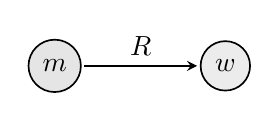
\begin{tikzpicture}[graph]
        \node[model] (M) {$m$};
        \node[world] (W) [right=of M] {$w$};

        \path[->] (M) edge node {$R$} (W);
    \end{tikzpicture}
    \caption{$mRw$ where $m$ is a model which represents a target world $w$}
    \label{fig:represent}
\end{figure}

\hypertarget{the-multiplicity-of-representational-models}{%
\subsection{The Multiplicity of Representational
Models}\label{the-multiplicity-of-representational-models}}

There are a wide array of different possible model-target representation
relationships. Each distinct relation is characterized by capturing
different aspects of the target and serving different purposes. The fact
that there are many ways to model any given target is widely established
in the literature. We care about this multiplicity because it means
different motivations for modeling lead to different models which relate
to their targets in unique ways. To illustrate this multiplicity, I'll
walk through a few models of the Earth, \(e\), which serve different
purposes thus represent their target in very different ways.

First, consider an educational representation \(R_{GEO}\) which is meant
to teach a student the natural geography of the planet, informing them
of how mountain ranges, lakes, and the sort fit on the planet. A globe
\(g\) can be a fantastic model of this, especially one that is textured
to add raised areas to represent the varying elevations on the planet.
Such a globe might even omit national boundaries to avoid cluttering the
display of geographic features. I'd argue these ``raised relief'' maps
do a fantastic job of conveying this info, so \(gR_{GEO}e\) might hold.
We could say that \(g\) is a model of \(e\) in this case.

However, \(g\) might be a terrible model of the Earth in other contexts.
For example, the globe \(g\) would be a decidedly suboptimal way to plan
a transcontinental railway through contested political boundaries.
Because \(g\) focused on natural features, it omitted political
boundaries entirely and almost certainly had smaller, yet exaggerated
bumps to represent mountain ranges. The missing boundaries would make it
difficult for planners to know where the railroad legally could be built
and the exaggerated features would be a very imprecise way of assessing
the potential engineering challenges of a route. Thus, planners might
prefer to use a set of topographical maps \(m\) with detailed elevation
contour lines and political boundaries for only the continent the
railroad is planned for. Thus, the model map set \(m\) does a great job
representing the features of the planet that are salient to railroad
planning so \(mR_{PLN}e\) holds to some extent.

However, the map set \(m\) is not a particularly educational experience
for the uninitiated. Giving a child a set of maps will not transmit the
overall shape of the earth nearly as well as the globe \(g\) did because
it is designed to give planners, who are ostensibly familiarly with the
overall geography of the area, the exact information they need to
complete a task. In this sense, the relations \(R_{GEO}\) and
\(R_{PLN}\) are in tension because both \(g\) and \(m\) satisfy one but
not the other. However, this tension is not inherent to models. Consider
a computer geographic model, \(c\), such as Google Earth. This system
might be both easy to use so a child can learn about the Earth's
geography and have enough information from detailed satellite and
elevation info for the planners to do their job too. Thus, \(c\) would
be a better representation by both \(R_{GEO}\) and \(R_{PLN}\). I put
all of these relations together in visual form in Figure
\ref{fig:globes} to help indicate this multiplicity.

\begin{figure}
    \centering
    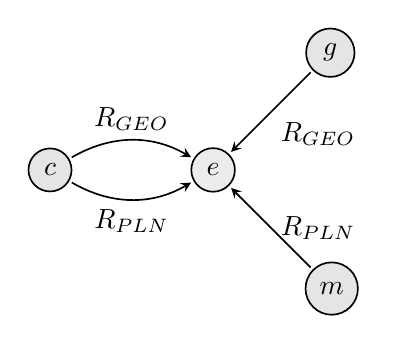
\begin{tikzpicture}[graph]
        \node[world] (e) {$e$};

        \node[model] (c) [left=of e] {$c$};
        \node[model] (g) [above right=of e] {$g$};
        \node[model] (m) [below right=of e] {$m$};

        \path[->] (g) edge node {$R_{GEO}$} (e);
        \path[->] (m) edge node[right] {$R_{PLN}$} (e);
        \path[->] (c) edge[bend right, below] node {$R_{PLN}$} (e);
        \path[->] (c) edge[bend left, above] node {$R_{GEO}$} (e);
    \end{tikzpicture}
    \caption{A globe $g$, set of planning maps $m$ and computer-based globe $c$ all represent the Earth in different, overlapping ways.}
    \label{fig:globes}
\end{figure}

\hypertarget{different-model-types}{%
\subsection{Different Model Types}\label{different-model-types}}

Given this multiplicity of models in general, I'll now sketch a few
situations in which someone could be thought of as using or creating a
representational model.

First, consider a drug toxicology study on a rat model. In this case,
the model is the rat and the target is a person. The researchers want to
know if a drug is toxic to people and they know that a large number of
things that are toxic to people are also toxic to rats and vice versa.
In this case, the model is a proxy for experimentation but might be
limited in terms of understanding what chemical effects actually cause
the toxicity, as it is easier to observe chemical reactions in a petri
dish than in some organ of a live rat.

Next, consider the classical mechanical mathematical model for the
motion of physical objects. This model is absurdly successful both at
capturing the true behavior of objects and of making that structure
understandable such that users of the theory can build on top of it. The
model takes the form of mathematical equations that relate quantities
like mass, acceleration force, and energy in experimentally-verified
ways. Thus, the model here is a set of equations like \(F=ma\) and
rules, like forces having equal and opposite reactions, which can be
useful in predicting physical behavior, like the trajectory of a cannon.
This model can also be useful as a foundation for other theories, like
statistical mechanics, where classical mechanical equations are combined
with other mathematical structures to model complicated regimes, like
diffusion. While this model creates many testable predictions, it isn't
a proxy for the target that is useful for experimentation in any
traditional sense. Where true experiments were run on the rat, the
equations and rules are mathematical and thus are analyzed
mathematically through analysis and proof, not thorough controlled
experiment and data collection.

Another type of model might be a simplified model of a complex
phenomenon. Consider the SIR epidemiological model framework as an
example. SIR models posit that people can be in one of three states:
susceptible, infected, and recovered. Other similar models add states
for exposed, but not infected or for a carrier who has recovered but is
still infective. This framework can be adapted to fit the
characteristics of a given disease. For example, influenza, transmitting
itself through the air, is much more adept at converting people from
susceptible to infected, so an epidemiologist creating an influenza
model would set the infection rate from S to I higher than that of a
sexually transmitted disease like HIV. This model framework, while
brittle, is capable of making good predictions about the dynamics of
epidemics, however, it strips away much of the complexity involved.
There is no differentiation between individuals: everyone is equally
likely to get the disease, everyone is equally likely to recover, etc.
Thus, this model is very good at capturing dynamics and making
predictions \footnote{I don't commit to these predictions being perfect.
  We think weather forecasting models are pretty good at making
  predictions even though forecasts are quite often wrong. Even if water
  doesn't end up falling from the sky, a prediction of 80\% chance of
  rain from a weather model tells us a lot about how that day might feel
  because it probably isn't clear and sunny if such a prediction is
  made. I'd argue we can think of SIR models the same way, where
  predictions are inaccurate, but usefully wrong by setting
  expectations.} in some cases, but doesn't capture any of the salient
mechanisms at play, and isn't a good way to study interventions alone.

For example, the differential equations view of infectious diseases only
models the \emph{rate} of infection, rather than the mechanism of
infection. Thus, according to the SIR model, a disease that spreads
through the air and one that spreads through the water might look
identical if they have the same infection rate. This is true even if the
mechanisms at play are quite different because of the model structure at
play. In this case, that model wouldn't be much use in evaluating which
mechanisms best interfere with the infection mechanism because that
aspect of the disease is left out of the SIR model.

\hypertarget{mathematical-models}{%
\subsection{Mathematical Models}\label{mathematical-models}}

Because simulations certainly have some relation to mathematical models
given making them involves typing mathematical formulas into a computer
at some level, I'll dedicate a bit more time to types of mathematical
models. My main goal here is to begin sketching a relationship between
complexity or simplicity and mathematical models. I'll argue that point
that while mathematical models can tackle complicated targets, they
inherently simplify.

Sometimes this simplification comes without compromising accuracy very
much at all, as is the case for mechanics. However, often it doesn't and
there is a notable tradeoff between the simplicity of the model and how
accurately it models its target system. The SIR model only models the
dynamics of a disease in a simplified sense; sometimes that
simplification is useful to produce accurate forecasts, but other times
it oversimplifies and misses key mechanisms at play.

While I'm not a mathematician or researcher primarily in the business of
formulating models, I'm going to take a stab at creating a plausible
story for why this is the case. Formulating a mathematical model
requires systematizing the target and finding mathematical structures
which model it well. This means that the modeler is beholden to the
language of mathematics when creating the model so if structures that
might model a target are unwieldy or non-existent, the modeler is forced
to simplify to something more tractable. Take the SIR model, for
example. It formulates an epidemic as a set of differential equations,
which oversimplifies in some sense. But, if we ask what it would take to
avoid this simplification, but keep everything in the language of math,
we wouldn't necessarily have a clear answer or next steps. Establishing
rigorous mathematical results, even for facts we are very sure are true,
can be a fraught and time-consuming endeavor. Consider,
\(P \stackrel{?}{=} NP\) problem, where we are so sure \(P \neq NP\)
that much of the modern world has been built around cryptography that
fundamentally assumes its truth, yet the problem remains open.

So, perhaps the language of mathematics fundamentally limits accounting
for complexity because of how difficult analytic work can be. While
mathematicians are always working to expand the bounds of what can be
analytically modeled with math, it is plausible, even probable, that
there will be many instances where the mathematical abstractions aren't
ideal and are difficult to work with. I'd wager these cases pop up
frequently when modeling very complex phenomena from the real world
because systemizing complexity, without oversimplifying, seems like an
inherently difficult problem. In these instances, is the modeling
researcher stuck waiting for mathematical results to catch up?

\hypertarget{computer-simulation-and-complexity}{%
\subsection{Computer Simulation and
Complexity}\label{computer-simulation-and-complexity}}

I offer simulation as a means of getting around a lack of mathematical
results to allow a modeler to embrace complexity where the math would
otherwise be intractable.

First, I should clarify exactly what I mean by ``simulation''. I adopt
Eric Winsberg's definition as ``a program which runs on a computer and
uses step-by-step methods to explore the approximate behavior of a
mathematical model'' \autocite{winsbergComputerSimulationsScience2019}.
This definition stresses both that simulations are based on mathematical
models and that they are typically time-dependent. The simulation
approximates, rather than mimics perfectly the model like an analytic
result would. A simulation doesn't give satisfactory proof, but can give
a pretty good idea of the truth of something.

To illustrate the difference, consider that the act of designing fast
algorithms for NP-hard problems feels hard; just look at the engineering
effort behind modern constraint satisfaction solvers! Given the amount
of time that has gone into working on speeding these things up and
consequently how hard the problem seems, we might get the impression
that \(P \neq NP\). This feeling, however, isn't proof, and establishing
the result analytically would probably require methods very different
than optimizing code which solves NP-complete problems. However, this
feeling also gives us confidence that allows us to tie cryptography to
NP-complete problems and feel secure that a P solution doesn't exist,
even if there is no formal proof.

Like the \(P \stackrel{?}{=} NP\) problem example, simulations give us
evidence, not proof. However, evidence alone is often sufficient and is
certainly much better than no understanding at all. Simulations are
imperfect, they approximate, they discretize, and they are inefficient
compared to analytic results. However, they form the backbone of
understanding complicated systems and are critical to weather
forecasting, engineering, and other fields where the math quickly gets
unwieldy due to inherent complexity. For example, understanding the
turbulent flow of air can be modeled mathematically by the Navier-Stokes
equations. However, these equations rarely can be used to attain exact
analytic solutions to the aerodynamics problems many engineers care
about. Thus, instead of being blocked by the lack of analytic progress,
engineers developed large scale computer simulations based around these
equations that provide a great heuristic for the aerodynamic forces a
car or plane would experience in the real world. However, they are not
sure to be right all the time so the simulated results are typically
verified experimentally using a physical model and a wind tunnel.

So, given this placement of simulation models, we might view them as
ways of reincorporating some of the complexity lost in translation from
world to mathematical model. The mathematical model might work great in
simple regimes and might be verified by experiments in those regimes.
However, because the world is complex, analytical solutions often
oversimplify certain targets. Simulation can be used to bridge this gap
on complicated targets by removing the analytical and computational
burden of building a complicated model.

\hypertarget{mechanisms-experimentation-and-explanation}{%
\section{Mechanisms, Experimentation, and
Explanation}\label{mechanisms-experimentation-and-explanation}}

Now that I've framed simulations as allowing simplified mathematical
models to become more complex to model more complicated targets more
accurately, I will discuss why we'd want to do this. A common question
should be shouldn't we want simple, understandable theories? A key
criterion for a scientific theory is a preference for simpler theories,
but it seems like simulation moves in the opposite direction. To see
why, I turn to physical, biological models, which I see as providing a
useful framework for understanding simulations. This section will
discuss mechanisms and explanations to serve as a basis for my later
analysis of simulations through the lens of mechanism. Thus, this
section will be a bit of a detour to build a foundation.

Traditional understandings of science often failed to account for
increasingly successful biological methodologies because they focused
too much on physics as the exemplar for science as a whole. To rectify
this, theories of science which center the process of examining and
thinking in terms of mechanisms, rather than theories, emerged to better
understand the scientific process in biology. In this section, I draw
from Carl Craver and James Tabery's article on the subject to hopefully
provide a consensus account of mechanism
\autocite{craverMechanismsScience2019}.

At a high level, I adopt Bechtel and Abrahamsen's definition of
mechanism:

\begin{quote}
A mechanism is a structure performing a function in virtue of its
component parts, component operations and their organization. The
orchestrated functioning of the mechanism is responsible for more than
one phenomena. \autocite{bechtelExplanationMechanistAlternative2005}
\end{quote}

This definition identifies the key parts of a mechanistic model:
phenomena, parts, causing, and organization.

The phenomena of a model, in the context of a mechanistic explanation,
is simply what is being explained by the behavior of a given mechanism.
We can take this in a causal sense as we developed earlier saying the
phenomenon is \emph{caused} by the mechanism. Phenomena and mechanisms
can be described in terms of their inputs and outputs. For example, an
engine (at a high level) takes in gas as an input and outputs rotational
energy and exhaust, so we could consider it a mechanism which explains
the observed phenomena associated with that energy conversion.

Mechanistic models are composed of one or more parts. How this
decomposition happens will vary a lot depending on the mechanism and how
it can naturally be divided. In the case of the engine example, the
engine is composed of pistons, spark plugs, timing belts, exhaust pipes,
and fuel injectors, among others. It is easy in this case to identify
the parts because the engine is engineered by people who design the
device to be easy to build, test, and understand. However, in scientific
examples, these divisions between parts can become less clear.

Next, these parts causally interact with one another. Because
mechanistic models seek to provide causal explanations, we call these
interactions \emph{causings}. For example, the spark plugs cause the
ignition of the gas mixture. A part may also cause multiple things, for
example, a piston both captures the energy from the combustion of the
gas mixture and pushes exhaust from that combustion out of the chamber.

Finally, the parts are organized such that phenomena emerge from their
combination. For example, any single part of the engine could not
convert gas to motion alone, but the arrangement of the parts in concert
creates the emergent phenomena of the car moving. Additionally, the same
part may show up multiple times in a mechanism as an engine often has
four, six, or eight identical cylinders.

If we combine all these parts and can break the phenomena down into
parts and understand how those parts relate and combine to \emph{cause}
the phenomena, we'd say we understand it pretty well. An engine is a
good example because engineers understand them very well given each of
these parts and relations were designed with the intent to produce the
given effect.

However, the mechanistic view doesn't just apply to things we've
designed. Mechanisms exist all around us as well. To pick a particularly
complicated example: the brain can be viewed as a mechanism. Say it
takes sensory data in and outputs movements (ignoring inner cognitive
states in this specific example). We might divide the brain into the
cerebrum, the cerebellum, and the brain stem and somehow categorize
interactions between these parts. While there isn't yet a satisfactory
understanding of consciousness in terms of mechanisms, other functions
do have such understandings. Neuroscientists can refer mechanistically
to the part of the brain which is connected to the eyes via optic nerves
as the visual cortex because it is responsible for vision. This
mechanistic responsibility follows from the observation that damage to
this bundle of nerves leads to degraded vision. However, this doesn't
mean that these nerves do nothing else but process visual stimuli,
simply that together they seem to be a key mechanism that enabled sight.
Because of this causal relationship, the bundle of nerves called the
visual cortex is usefully understood, studied, and referred to as a
mechanistic unit \footnote{Often these mechanistic understandings are
  very difficult to come by. Thus, it is important to note that things
  that seem very difficult to understand mechanistically given current
  knowledge and experimental methods could have very compelling
  mechanistic understandings. To see this, consider the striking example
  of microprocessors. A team of researchers tried to dissect a
  microprocessor using the first principles research techniques of
  neuroscience to generate a clean-sheet mechanistic understanding.
  Despite the microprocessor being man-made and mechanistically
  understood by the engineers who painstakingly organized it into
  functional units, the research team had trouble reaching any sort of
  mechanistic understanding. Because the researchers were limited in
  their ways of observing and manipulating the microchip to those used
  by neuroscientists, they couldn't understand enough of the chip to
  generate a compelling mechanistic understanding
  (\autocite{jonasCouldNeuroscientistUnderstand2017}).}.

To expand on the process of understanding mechanisms, it is important to
consider the manipulability account of causation that underpins much of
this theoretical work on mechanism. The idea, most recently advocated
for by James Woodward, is that establishing causal relationships can be
done by manipulating some part of a mechanism and observing that the
manipulation resulted in a different observation. Essentially, if a
causing mechanism \(C\) truly causes a phenomenon \(P\), then inhibiting
\(C\) should make \(P\) go away. Conversely, inserting \(C\) into a
mechanism should cause \(P\)
\autocite{woodwardScientificExplanation2019}.

This theory follows the language used in many biological settings, but
presents a very general framework for experimentation. In a biological
experiment, often the researcher will get two groups of organisms,
modify some mechanism in one of the groups, then compare the two. For
example, to establish that some gene plays a role in causing some
phenomena a researcher might use a gene knockout to render the gene of
interest inactive. In this case, if the phenomena changes, we have good
reason to believe that gene is a causing in the mechanistic sense.

An important feature of this theory of explanation is that the ability
to manipulate is critical to reaching understanding. If we don't have
the means to knock out that gene, we can't hope to get a mechanistic
explanation in this sense \footnote{There is plenty of literature on
  cases where causation may be inferred without experiment
  \autocite{hitchcockCausalModels2019}, however, this thesis focuses on
  the experimental approaches. Causal inference is a fantastic
  possibility because experimentation is hard, however, many
  explanations don't have the right structure to infer causation. In
  these instances, we'd still need to run experiments. Furthermore,
  scientists, for better or for worse, rely heavily on experimentation
  now, so that seems a natural place to start.}.

\hypertarget{experimentation-on-mechanistic-models}{%
\section{Experimentation on Mechanistic
Models}\label{experimentation-on-mechanistic-models}}

Because it is often hard, expensive, or unethical to experiment on
certain targets of interest, researchers often decide to manipulate
models instead. Because there is only one extremely large atmosphere,
climate scientists manipulate computational models because direct
manipulation of the atmosphere is extremely expensive and lacks any sort
of control group. Similarly, it would be unethical to experiment with a
human's genes to establish causal explanations of genetic mechanisms, so
biologists experiment on mice, rats, and other organisms with mechanisms
of interest that are known to be similar to those in humans \footnote{There
  are still many ethical issues at play here and not everyone is
  convinced that this experimentation is a moral practice. That being
  said, there are established ethical guidelines for this research and
  it is a fairly mainstream practice at this point that has been very
  productive for research.}.

Using an animal model for experimentation works because:

\begin{enumerate}
\def\labelenumi{\arabic{enumi}.}
\tightlist
\item
  The animal is presumed to have similar mechanisms of interest to the
  target organism.
\item
  The animal's mechanism can be more easily manipulated than the
  target's
\end{enumerate}

If the mechanisms aren't similar, the findings won't translate to the
target and if the model isn't more manipulable than the target, the
experimenter might as well just experiment directly on the target.
Stipulation one may be viewed as a prerequisite, while stipulation two
sets up the cost-benefit tradeoff of the model. What the experimental
model loses in applicability, it must make up for in ease of
manipulation for it to make sense.

\hypertarget{example-in-vitro-vs-in-vivo-models}{%
\section{\texorpdfstring{Example: \emph{in-vitro} vs \emph{in-vivo}
Models}{Example: in-vitro vs in-vivo Models}}\label{example-in-vitro-vs-in-vivo-models}}

Experimental models can vary in the level of manipulation they allow
for. The level of manipulation allowed for often comes at the expense of
the transportability of an explanation if the model mechanism diverges
too much from the target. Thus, scientists who use models to experiment
on must also make an argument that the model is an effective analog by
follow-up tests on the target directly, as in clinical trials of drugs,
or simply careful experimental design. The more manipulated a model is
by the researcher, the more argumentation is necessary to be sure that
the model actually replicates the target.

An example of this trade-off is the distinction between \emph{in-vivo},
and \emph{in-vitro} experimental methods. An \emph{in-vitro} model can
be a sample of tissue from an animal that has been removed from that
animal for experimentation where an \emph{in-vivo} model would
experiment on the animal directly. The \emph{in-vitro} model is
relatively easy to modify because it is constructed by the researcher,
where the \emph{in-vivo} model's environment is set by the organism
being experimented on.

For example, early analysis of the electrical properties of the neuron
were discovered using \emph{in-vitro} squid neuron models. Marine
biologists and biophysicists would dissect giant squids, extract their
axons, place them in a bath of saline solution and hook electrodes up to
them. This allowed for intricate electrical manipulation by sending
small pulses of current through the neuron to trigger action potentials
to propagate through the neuron. These electrodes also make in-depth
measurements of electrical properties easy. However, the researcher had
to deal with the concern that the observed properties stemmed from the
experimental setup and didn't actually occur when the neurons are part
of the larger organism.

Thus, a researcher could use an \emph{in-vitro} model to deeply analyze
some mechanism, then confirm it with an \emph{in-vivo} study that
verifies the phenomena observed \emph{in-vitro} can be observed
\emph{in-vivo}, though perhaps with a more complicated experimental
setup. In this sense, the \emph{in-vitro} models can be viewed as more
exploratory models that allow for easier manipulation which facilitates
more trial and error. A promising result found in exploratory
\emph{in-vitro} studies could then be confirmed in a hypothesis-based
\emph{in-vivo} study.

\hypertarget{computational-simulation-and-manipulative-experimentation}{%
\section{Computational Simulation and Manipulative
Experimentation}\label{computational-simulation-and-manipulative-experimentation}}

To return to simulations, I argue that experimental simulations can be
thought of much like \emph{in-vitro} experimental models in biology.
They both provide a very complex model environment that can mimic
mechanism when done right and allow for a lot of manipulation to
facilitate the generation of explanation. However, like \emph{in-vitro}
models, this flexibility raises questions about the transportability of
explanations from models.

The goal for the rest of this thesis is to show how mathematical models
can be made into simulations that mimic the complexity of its target
more directly and more convincingly. This will make models more complex,
but in doing so make the proxy relationship between model and target
easier to see to better contextualize results and make the
transportability of claims more plausible.
